% Appendix Template

\chapter{Results of experiment 2.5} % Main appendix title

\label{Appendix2-5} % Change X to a consecutive letter; for referencing this appendix elsewhere, use \ref{AppendixX}

\begin{figure}[th]
\centering
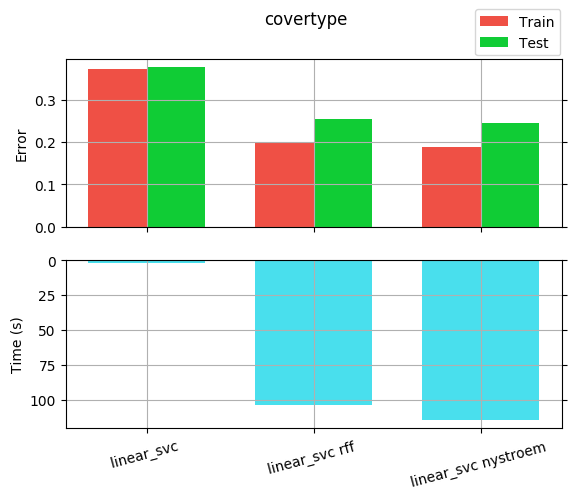
\includegraphics[scale=\imgscale]{Figures/2_5/covertype}
\decoRule
\caption[2.5 covertype]{Linear-SVC with RFF and \Nys}
\label{fig:2_5_covertype}
\end{figure}

\begin{figure}[th]
\centering
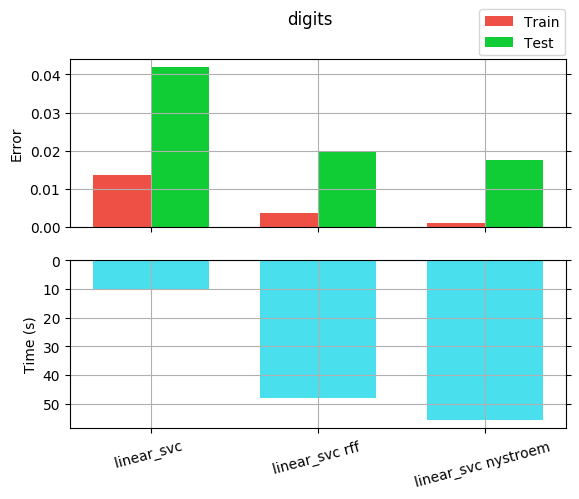
\includegraphics[scale=\imgscale]{Figures/2_5/digits}
\decoRule
\caption[2.5 digits]{Linear-SVC with RFF and \Nys}
\label{fig:2_5_digits}
\end{figure}

\begin{figure}[th]
\centering
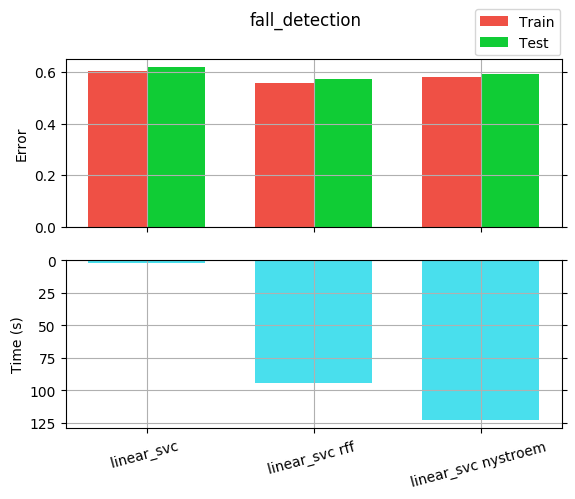
\includegraphics[scale=\imgscale]{Figures/2_5/fall_detection}
\decoRule
\caption[2.5 fall\tu detection]{Linear-SVC with RFF and \Nys}
\label{fig:2_5_fall_detection}
\end{figure}

\begin{figure}[th]
\centering
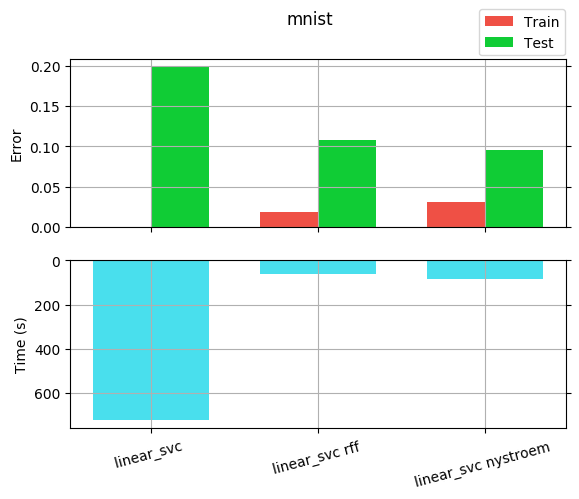
\includegraphics[scale=\imgscale]{Figures/2_5/mnist}
\decoRule
\caption[2.5 mnist]{Linear-SVC with RFF and \Nys}
\label{fig:2_5_mnist}
\end{figure}

\begin{figure}[th]
\centering
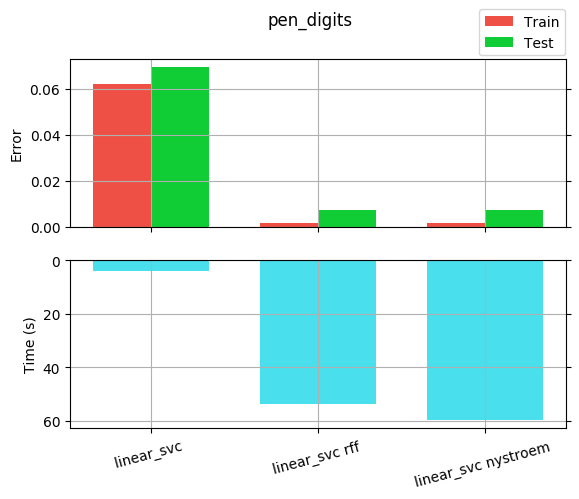
\includegraphics[scale=\imgscale]{Figures/2_5/pen_digits}
\decoRule
\caption[2.5 pen\tu digits]{Linear-SVC with RFF and \Nys}
\label{fig:2_5_pen_digits}
\end{figure}

\begin{figure}[th]
\centering
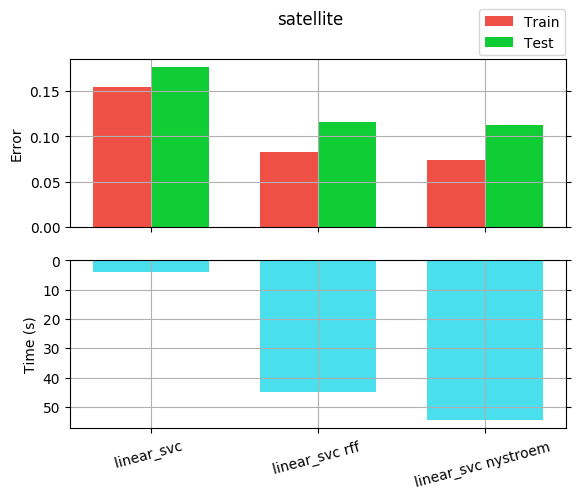
\includegraphics[scale=\imgscale]{Figures/2_5/satellite}
\decoRule
\caption[2.5 satellite]{Linear-SVC with RFF and \Nys}
\label{fig:2_5_satellite}
\end{figure}

\begin{figure}[th]
\centering
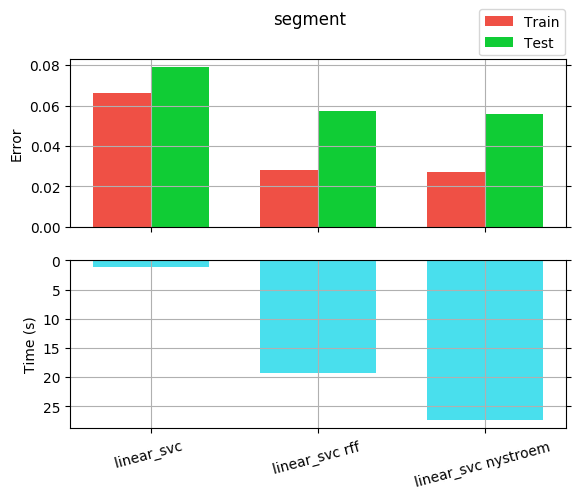
\includegraphics[scale=\imgscale]{Figures/2_5/segment}
\decoRule
\caption[2.5 segment]{Linear-SVC with RFF and \Nys}
\label{fig:2_5_segment}
\end{figure}

\begin{figure}[th]
\centering
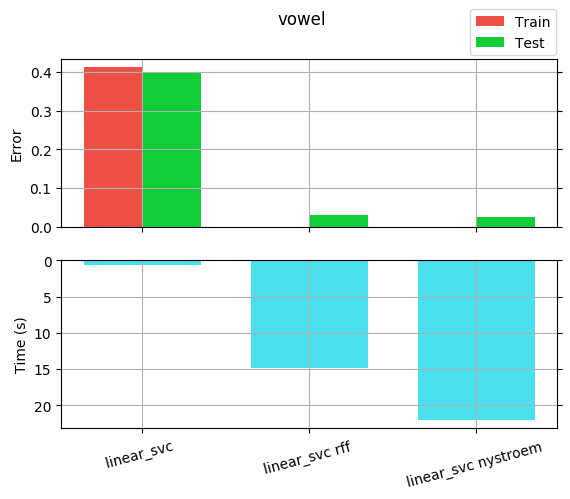
\includegraphics[scale=\imgscale]{Figures/2_5/vowel}
\decoRule
\caption[2.5 vowel]{Linear-SVC with RFF and \Nys}
\label{fig:vowel}
\end{figure}
